\documentclass[tikz,border=10pt]{standalone}
\usepackage{amsmath}
\usepackage{tikz}
\usetikzlibrary{arrows.meta, positioning, angles, quotes, decorations.markings, calc}

\begin{document}

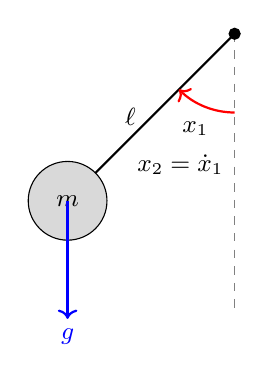
\begin{tikzpicture}[
  mass/.style = {circle, draw, fill=gray!30, minimum size=1cm},
  string/.style = {thick},
  anglemark/.style = {draw, ->, thick, red},
  force/.style = {->, thick, blue},
  arrow/.style = {thick, -{Latex[width=2mm]}},
  every node/.style = {font=\small}
]

% Parameters
\def\L{3}
\def\theta{45} % degrees

% Coordinates
\coordinate (pivot) at (0,0);
\coordinate (bob) at ($(pivot) + (\theta:-\L)$);

% Draw dashed vertical equilibrium line
\draw[dashed, gray] (pivot) -- ++(270:\L+0.5);

% Draw the pendulum
\draw[string] (pivot) -- (bob);
\node[mass] at (bob) {$m$};

% Draw pivot
\filldraw[black] (pivot) circle (2pt);

% Angle arc from vertical to pendulum line (270° to 270 - θ)
\draw[anglemark] (pivot) ++(270:1) arc[start angle=270, end angle={270 - \theta}, radius=1];
\node at ($(pivot)+({270 - 0.5*\theta}:1.3)$) {$x_1$};
\node at ($(pivot)+({270 - 0.5*\theta}:1.8)$) {$x_2 = \dot{x}_1$};

% Gravity force
\draw[force] (bob) -- ++(0,-1.5) node[below] {$g$};

% Length label
\path (pivot) -- node[midway, left=2pt] {$\ell$} (bob);

\end{tikzpicture}

\end{document}
